\documentclass[a4paper,12pt,twoside,dvipdfmx]{jreport} % A4 用紙,12pt フォント

% =========================== use package ================================== %
\usepackage[inner=25mm,outer=25mm,top=40mm,bottom=25mm]{geometry} % 余白の設定
\usepackage{titlesec} % 章タイトルのフォーマット
\usepackage{fancyhdr} % ヘッダーとフッターの設定
\usepackage{pdfpages} %pdf追加用

\usepackage{csquotes} % 日本語引用のためのパッケージ
\usepackage[T1]{fontenc} % 「OT1エンコーディングでは\kが使えない」とかいう意味わかんないコンパイルエラー解消用 (note → https://www.notion.so/15741bdf4d89808fae3ef68818d9452b?pvs=4#15c41bdf4d89803bbbc9c3bf517435ca)
\usepackage[japanese]{babel} % 参考文献の表示を「参考文献」にする
\usepackage[backend=biber, sorting=none, maxbibnames=99]{biblatex} % 参考文献用, sorting=noneで引用順を保持, maxbibnames=99で最大99個のauthorを表示
\addbibresource{ref.bib} %.bibのファイル名指定

\renewcommand{\baselinestretch}{1.2} % 行間を1.2倍に設定

% svgをダイレクトに入れられるようにする
\usepackage{svg} 

% 図をmatrix形式で表示するためのパッケージ
\usepackage{tabularx} % プリアンブルに追加
\usepackage{array} % プリアンブルに追加

\usepackage{amsmath} % 数式を綺麗に表示するためのパッケージ
\usepackage{bm} % 太文字
\DeclareMathOperator*{\argmax}{argmax} %数式でのargmaxの定義  使い方: \mathop{\arg\max}_{i}

\usepackage{hyperref} % リンクを有効にする

% キャプション設定 -------------------------------------- %
\usepackage{caption}
\usepackage{subcaption} % サブキャプション
\captionsetup{font=small}

% 表のラベルをTab.に変更
\DeclareCaptionLabelFormat{tab}{\textbf{Table.~#2}}
\captionsetup[table]{labelformat=tab}

% 図のラベルをFig.に変更
\DeclareCaptionLabelFormat{fig}{\textbf{Fig.~#2}}
\captionsetup[figure]{labelformat=fig}
% キャプション設定 -------------------------------------- %

% ========================================================================== %


% ============================ 独自コマンドの定義 ===========================%
\newcommand{\figref}[1]{Fig. \ref{#1}}
\newcommand{\tabref}[1]{Table. \ref{#1}}
\newcommand{\eqrefc}[1]{Eq. \ref{#1}}
% ========================================================================= %


% ============================ header & footer ============================ %
\pagestyle{fancy}
\fancyhf{}
% 偶数ページの設定
\fancyhead[LE]{\leftmark} % 左ヘッダに章名
\fancyhead[CE]{}
\fancyhead[RE]{}
\fancyfoot[CE]{\thepage}

% 奇数ページの設定
\fancyhead[LO]{\rightmark} % 左ヘッダに節名
\fancyhead[CO]{}
\fancyhead[RO]{}
\fancyfoot[CO]{\thepage}
% ========================================================================== %


% ========================================================================== %
% 章タイトルを中央揃えに設定し、「第1章」の形式にする
\titleformat{\chapter}[display]
{\normalfont\huge\bfseries\centering} % フォントスタイルと中央揃え
{第\arabic{chapter}章}{20pt}{\Huge}
% ========================================================================== %


% ================================ document ================================ %
\begin{document}


% 表紙pdfの挿入
\includepdf[pages=-,fitpaper=true]{Other/myhyousi.pdf}
\cleardoublepage


% タイトル
\begin{titlepage}
    \begin{center}
        {\fontsize{24pt}{24pt}\selectfont  修士学位論文}
        \vspace{3cm}
  
        {\fontsize{20pt}{20pt}\selectfont \textbf{膜電位ダイナミクス安定化による}}
        \vspace{0.5cm}

        {\fontsize{20pt}{20pt}\selectfont \textbf{Spiking Neural Networkの}}
        \vspace{0.5cm}

        {\fontsize{20pt}{20pt}\selectfont \textbf{入力時系列変化に対する頑健性の向上}}
        \vspace{7cm}

        {\fontsize{18pt}{18pt}\selectfont 令和6年度} 
        \vspace{0.5cm}

        {\fontsize{18pt}{18pt}\selectfont (令和7年2月1日 提出)} 
        \vspace{3cm}

        {\fontsize{18pt}{18pt}\selectfont 東北大学大学院工学研究科}
        \vspace{0.5cm}

        {\fontsize{18pt}{18pt}\selectfont ロボティクス専攻}
        \vspace{1.0cm}

        {\fontsize{18pt}{18pt}\selectfont 平野 貴也}
    \end{center}
  \end{titlepage}
\cleardoublepage


% 英語アブスト
\pagestyle{empty}

\begin{center}
    Muscle Roulette! Startt! Muscle Warp! ~Nnnnnn..! Nuun! Nuun!
\end{center}
\vspace{10mm}
\begin{center}
    Shoji Nakayama
\end{center}
\vspace{10mm}

\begin{center}
    Abstract
\end{center}
\vspace{10mm}

Nakayamakinnikun (September 17, 1978) is a Japanese male comedian, YouTuber, and bodybuilder. 
Born in Higashi Ward, Fukuoka City, Fukuoka Prefecture, he was a member of Yoshimoto Kogyo from 2000 to 2021 and freelance after 2022.
His real name is Shoji Nakayama.
He graduated from Wahirohigashi Elementary School in Fukuoka City, Wahirokaoka Junior High School in Fukuoka City, and Fukuoka Institute of Technology High School (now Joto High School attached to Fukuoka Institute of Technology).He had a muscular physique since his school days, but was more passionate about basketball than bodybuilding at that time.
He started muscle training at LBGYM in Kashii during his high school years.After becoming a TV personality, he visited LBGYM in 2005 and 2020 for a commercial TV program in Fukuoka.The program was aired on RKB Mainichi Broadcasting and TNC TV Nishinihon.
One of her classmates in high school was Motoei Kusakabe, a female judoist and bronze medalist at the Sydney Olympics.After graduating from high school, she entered Yoshimoto Sogo Gakuin (NSC) Osaka School as a 22nd year student [2][5].Before entering NSC, he appeared on the October 30, 1998 broadcast of Asahi Broadcasting Corporation's "Tantei!Night Scoop" on October 30, 1998 [Note 1] [Note 2].His classmates at NSC include Super Maradona, Kazunobu Kubota (Torosomon), and King Kong.After graduating from NSC in 2000, he debuted with Yoshimoto Kogyo as "Nakayamakini-kun," a pin comedian who performs gags using muscles[2].His godfather was Takayuki Haranishi (FUJIWARA), who was also his senior at NSC, but the name he initially invented was simply "Kinnikun" without "Nakayama." In 2001, he joined Yoshimoto Shinki Gekijou, where he played a clerk and a henchman of a yakuza gang.After completing a series of material in which he talks while using his muscular body to show off his muscles, he reports to his older brother (or employer, etc.), "I did all I had to do!I've done all I can do!"[Note 3] In January 2003, he won the judges' special award at the 24th ABC Comedy Newcomer Grand Prix.In 2006, he invented a new character, "Captain Bomber," who was supposed to be "a man from North Carolina who came to Japan to introduce American culture," and made it to the finals of the R-1 Grand Prix that same year.On this occasion, he placed a portrait of Nakayamakin on stage and performed his material as a different person from Kinnikun (even though he denied being called Kinnikun) [Note 4].When asked by his co-star Shinya Ueda (Kurimuchu) about his appearance on Asahi Broadcasting Corporation TV's "Gold Medal of Laughter" under the name Captain☆Bomber, he stubbornly denied that he was Nakayamakini-kun.In the Shinkigeki theater to which he belongs, he has been pushing "Captain Bomber" to the forefront and has started an event "Shinkigeki Bomber!He was also appointed as the image character of "Puururando RiO" at Misaki Park in Misaki Town, Sennan County, Osaka Prefecture, and his name recognition was greatly enhanced.Around the same time, he used his physical training to participate in the then-popular TBS "Who's the Strongest Man?The Fierce Muscle Battle!He has appeared in sports specials such as "The Sportsman No. 1 Championship" and has achieved a number of good results (see below).


\clearpage
\pagestyle{fancy} %abstract追加
\cleardoublepage


% 目次
\pagenumbering{roman} % ページ番号をローマ数字に設定
\setcounter{page}{1}
\tableofcontents % 目次を生成
\listoffigures %図目次
\listoftables %表目次


% 本文
\cleardoublepage % 奇数ページから始める
\pagenumbering{arabic} % ページ番号をアラビア数字に設定
\setcounter{page}{1} % ページ番号を1にリセット
\chapter{序論}
\section{来歴}
福岡市立和白東小学校、福岡市立和白丘中学校、福岡工業大学附属高等学校(現・福岡工業大学附属城東高等学校)を卒業\cite{wiki}。

学生時代から筋肉質な体格だったが、当時はボディビルよりもバスケットボールに熱中していた。高校時代に香椎のLBGYMで筋トレを始める。

タレントになった後、福岡の民放番組で2005年と2020年にそのLBGYMを来訪。その様子がRKB毎日放送とTNCテレビ西日本で放映された。

高校時代の同級生には女子柔道家でシドニーオリンピック銅メダリストの日下部基栄がいる。

高校卒業後は吉本総合芸能学院 (NSC) 大阪校に22期生として入学する[2][5]。なお、入学前に1998年10月30日放送の朝日放送テレビ『探偵!ナイトスクープ』の依頼「世界一指を早く回せる男」に出演している[注 1][注 2]。これはバスケットボール選手が指を回す際の仕草である。NSCの同期には、スーパーマラドーナ・久保田かずのぶ(とろサーモン)・キングコングなどがいる。

\begin{figure}[htbp]
  \centering
  \includegraphics[width=0.5\textwidth]{Chapter1/figures/image.png}
  \caption{キャプテン☆ヒーロー}
  \label{fig:my_label}
\end{figure}

\section{先行研究}
こうしたSNNにおける時間的特性の課題に対して, 先行研究では時定数を学習可能とし, その多様性を実現することが多く行われている\cite{dhsnn, yin2020effective, paramsnn}.
本節では, ニューラルネットワークの重みとバイアスと同様に, 時定数を学習可能とした手法について述べる.
さらに, 1つのニューロンに対して複数の時定数を割り当てることで, SNNの時間的特性を向上させた手法について記述する.

\subsection{Parametric-SNN}
前述の通り, LIFモデルで構成されたSNNの学習アルゴリズムでは, 膜電位の時定数はハイパーパラメータとして扱われる.
そのため, SNNの学習ではニューロン間の接続重みとバイアスのみが最適化される.
しかし, 時系列入力に対するSNN内のニューロンダイナミクスは, その時定数による影響を無視できない.
ある単一のニューロンにおける入力と膜電位の関係の模式図を\figref{fig:lif}に示す.
ニューロンは膜電位$V$を持ち, その値は前方のニューロンからの入力$I$によって変化する.
さらに, その変化量は前方のニューロンの接続重み$w$とそのニューロンの時定数$\tau$に依存する.
また, ニューロンに定常入力が加わったときの膜電位の時間変化を\figref{fig:liffigure}に示す.
ここで, 曲線origin(青線)は時定数$\tau$と重み$w$が基準値のときの膜電位の時間変化を表す.
一方で, $w^+, \tau^+$はそれぞれ重みと時定数が基準値より大きい場合の膜電位の時間変化を表す.
また, $w^-, \tau^-$はそれぞれ重みと時定数が基準値より小さい場合の膜電位の時間変化を表す.
\figref{fig:liffigure}より, ニューロンの接続重み$w$だけでなく, 時定数$\tau$の値によっても膜電位の収束速度が変化することがわかる.
このことから, 時定数を学習可能とすることで, SNNの時間表現能力の向上が期待される.
\begin{figure}[htbp]
    \centering

    \parbox{1.0\textwidth}{
        \centering

        \begin{minipage}{0.243\textwidth}
            \includegraphics[width=1.0\textwidth]{Static/chap1_paramsnn_neuronmodel.pdf}
            \subcaption{LIFモデル}
            \label{fig:lif}
        \end{minipage}
        \hspace{0.02\textwidth}
        \begin{minipage}{0.657\textwidth}
            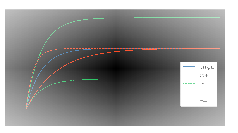
\includegraphics[width=1.0\textwidth]{Static/chap1_paramsnn_volttrj.pdf}
            \subcaption{LIFモデルにおける膜電位変化}
            \label{fig:liffigure}
        \end{minipage}

        \caption[LIFモデルの模式図と膜電位の時間変化]{
            \cite{paramsnn}
            (a) LIFニューロンモデルの模式図. $I, V$はそれぞれニューロンへの入力と膜電位. 
            $w, \tau$はそれぞれニューロン間の接続重みと時定数. 
            (b) ニューロンに定常入力が加わったときの膜電位の時間変化. 
            $+, -$はそれぞれのパラメータの大小を表す.
        }
    }
\end{figure}

Fangらは, このようなSNNの時定数を学習可能としたアルゴリズムとしてParametric-SNNを提案した\cite{paramsnn}.
Parametric-SNNでは, ニューロンの重み$w$と同様に時定数$\tau$が学習中に最適化される.
そのため, 事前に時定数をハイパーパラメータとして設定する必要がない.
また, SNNの同じ層ではニューロン間の時定数が共有される.
これは, 脳における隣接するニューロンは類似の時間特性を持つ特徴を反映しており, 生物的妥当性が高い.
一方, 異なる層間では時定数は共有されず, 異なる値を持つ.
これによって, SNNが多様な時間的特性の学習が可能となる.
結果として, Parametric-SNNは従来のLIFモデルを用いたSNNよりも画像認識, 動画認識タスクにおいて高いパフォーマンスを発揮した (\tabref{tab:paramsnn:result1}).
さらに, その学習の収束速度も向上することが示された (\figref{fig:paramsnn:traincurve}).
\begin{table}[htbp]
    \centering
    \caption[Parametric-SNNのパフォーマンス]{
        Parametric-SNNのパフォーマンス\cite{paramsnn}.
        タスクは画像認識, 動画認識のベンチマークテスト. 
        $\tau$は学習前の時定数の初期値を表す.
    }
    \label{tab:paramsnn:result1}
    {\small %12ptだとはみ出るので小さく
    \begin{tabular}{ccccc}
        \hline
        Model & Fashion-MNIST & CIFAR-10 & CIFAR10-DVS & DVS128 Gesture\\
        \hline
        Parametric-SNN ($\tau_0=2$) & \textbf{94.38 \%} & \textbf{93.50 \%} & \textbf{74.80 \%} & \textbf{97.57 \%}\\
        SNN ($\tau=2$) & 94.17 \% & 93.03 \% & 73.60 \% & 96.88 \%\\
        \hline
        Parametric-SNN ($\tau_0=16$) & \textbf{94.65 \%} & \textbf{93.23 \%} & \textbf{70.50 \%} & \textbf{92.01 \%}\\
        SNN ($\tau=16$) & 94.47 \% & 47.50\% & 62.40 \% & 76.74 \%\\
        \hline
    \end{tabular}
    }
\end{table}

\begin{figure}[htb]
    \centering
    \includegraphics[width=0.8\textwidth]{Static/chap1_paramsnn_traincurve.pdf}
    \caption[Parametric-SNNとSNNの学習曲線]{
        Parametric-SNNとSNNの学習曲線\cite{paramsnn}.
        LIF, PLIFはそれぞれ従来のLIFモデル, Parametric-SNNを表す.
        $\tau$が同じSNNとParametric-SNNを比較したとき, Parametric-SNNの方が収束が速い.
    }
    \label{fig:paramsnn:traincurve}
\end{figure}


\subsection{DH-SNN}
Parametric-SNNでは, 時定数を学習可能とすることで, ニューロンダイナミクスの時間特性に対して多様性を与えた.
しかし, ニューロンへの入力に対する時間的特性については考慮されていない.
\figref{fig:single:neuron}に単一ニューロンの模式図を示す.
ニューロンの内部状態$u$は, ニューロンへの入力$i$によって変化する.
ここで, 入力$i$は前方に接続されたニューロンからの信号が直接伝達されるわけではない.
枝枯れした樹状突起と呼ばれる構成要素が前方のニューロンからの信号を受け取る.
その後, それぞれの樹状突起からの信号の総和がニューロンへの入力となる.
脳では, ニューロンの多様な時間的特性に加えて, それぞれの樹状突起も異なる時間的特性を持つことで, 複雑な時間表現を可能にしている.
しかしながら, LIFモデルや先行研究では, この樹状突起の時間特性の多様さは考慮されていない.
\begin{figure}
    \centering

    \parbox{1.0\textwidth}{
        \centering

        \begin{minipage}{0.42325\textwidth}
            \includesvg[width=1.0\textwidth, inkscapelatex=false]{Static/chap1_dhsnn1}
            \subcaption{単一ニューロン}
            \label{fig:single:neuron}
        \end{minipage}
        \hspace{0.02\textwidth}
        \begin{minipage}{0.477\textwidth}
            \includesvg[width=1.0\textwidth, inkscapelatex=false]{Static/chap1_dhsnn2}
            \subcaption{DH-SNNにおける単一ニューロンの概要図}
            \label{fig:dhsnn}
        \end{minipage}

        \caption[DH-SNNにおける単一ニューロンの模式図]{
            \cite{dhsnn}
            (a) 単一ニューロン. $i, u$はそれぞれニューロンへの入力と膜電位. 
            ニューロンへの入力$i$は, 枝分かれした樹状突起からの信号の総和としてモデル化される.
            (b) DH-SNNにおける単一ニューロンの概要図.
            $\alpha_i$はそれぞれの樹状突起の持つ時定数を表す.
            $\beta$はニューロンの持つ時定数を表す.
        }
    }

    % \vspace{0.5cm}

    % \parbox{1.0\textwidth}{
    %     \centering
    %     \includesvg[width=0.9\textwidth, inkscapelatex=false]{Static/chap1_dhsnn3}
    %     \label{fig:dhsnn:network}
    %     \caption[DH-SNNのネットワーク構造]{
    %         DH-SNNのネットワーク構造\cite{dhsnn}
    %     }
    % }
\end{figure}

Zhengらは, このような樹状突起の時間特性の多様さを表現するDH-SNNを提案した.
\figref{fig:dhsnn}にDH-SNNにおける単一ニューロンの概要図を示す.
時定数$\beta$を持つ1つのニューロンに対して, $d$個の樹状突起を接続する.
さらに, それぞれの樹状突起に対して$\alpha$で表される時定数を割り当てる.
このニューロンの時定数$\beta$と樹状突起の時定数$\alpha$を学習することで, より複雑な時間情報の学習が可能になる.
また, DH-SNNは長期の時間依存関係の学習にもその有効性が示された.
通常, ニューロンの膜電位はその活性によって電気パルス信号を出力すると, その状態は初期状態にリセットされる.
そのため, LIFモデルは長期の時間関係の記憶が困難とされている.
一方, 樹状突起ではそのリセットが生じないため, より長期の時間関係の学習が可能となる.
DH-SNNを用いることで, 音声認識や動画認識, 脳波認識において, 通常のSNNと比較して高いパフォーマンスを発揮した(\figref{fig:dhsnn:voice}, \figref{fig:dhsnn:brain}).
\begin{figure}
    \centering

    \parbox{1.0\textwidth}{
        \centering

        \begin{minipage}{0.5336\textwidth}
            \includesvg[width=1.0\textwidth, inkscapelatex=false]{Static/chap1_dhsnn4}
            \subcaption{音声認識}
            \label{fig:dhsnn:voice}
        \end{minipage}
        \hspace{0.02\textwidth}
        \begin{minipage}{0.3663\textwidth}
            \includesvg[width=1.0\textwidth, inkscapelatex=false]{Static/chap1_dhsnn5}
            \subcaption{脳波認識}
            \label{fig:dhsnn:brain}
        \end{minipage}

        \caption[DH-SNNにおける精度比較]{
            \cite{dhsnn}
            (a) 音声認識タスク精度比較.
            灰色が従来のSNN, 青・緑・赤色がDH-SNNを表す.
            DH-SNNにおける色の薄さは樹状突起における時定数の学習の有無を表す.
            (b) 脳波認識タスク精度比較.
            青色が従来のSNN, その他の色がDH-SNNを表す.
            branchの数は1ニューロンから分岐する樹状突起の数を表す.
        }
    }
\end{figure}

\section{東京進出}
2011年2月2日、3年間の留学を終えて正式に帰国し、芸人に復帰すると共に東京進出の意向を明らかにした[13]。同年12月31日、日本テレビ『ダウンタウンのガキの使いやあらへんで!』の年越企画「笑ってはいけないシリーズ」の『絶対に笑ってはいけない空港24時』に出演。また、2013年には同シリーズの『絶対に笑ってはいけない地球防衛軍24時』内で松方弘樹が演じる防衛軍長官によって松本人志(ダウンタウン)にコードネームとして「まつもときんに君」が使用された。

2012年7月4日、映画『アベンジャーズ』のイベントに出演し、縁の深い八木真澄(サバンナ)の結婚式についての話題から自身が25歳のベルギー人女性と交際中であることを明かした[14]。

2014年5月、5人座長体制の新喜劇で座長を務める1人である小籔千豊の東京新喜劇公演に招集され、日替わりゲストとして出演した[15]。同年には同じく小籔の主催する「KOYABU SONIC 2014 FINAL」にも出演した[16]。

2019年9月、特撮テレビドラマ『仮面ライダーゼロワン』第1話「オレが社長で仮面ライダー」でヒューマギア(人型ロボット)・腹筋崩壊太郎役を演じると共にその怪人態・ベローサマギアの声も演じ、その役名と熱演ぶりから放送当日のTwitterでトレンドに入るほどの話題となった[17]。また、人々を笑わせることに喜ぶ同キャラクターが怪人化させられて悲壮な最期を遂げるという展開にちなむ単語「腹筋崩壊太郎ロス」が合わせてトレンド入りを果たしたことに、なかやまも感謝している[18][19]。後に、自身のYouTubeチャンネル『ザ・きんにくTV 【The Muscle TV】』のサブチャンネルで明かしたところによれば、オファーを受けた当初は驚いて令和初の怪人ということからも演技への不安にかられたが、役名を見て良い意味で肩(僧帽筋)の力が抜け、撮影の際にはバラエティ番組とは違った現場の雰囲気を楽しんだという[20][21]。また、後年のインタビューによれば、『ゼロワン』第1話の放送当日はオールジャパンフィジークの予選に出場していたため、予選中には知人からトレンド1位を知らせるLINEが多々来ていたという[22][2][注 7]。また、腹筋崩壊太郎の決め台詞「腹筋パワー!」や着用していたサスペンダーは当初には無く、前者はリハーサルの際に監督からの依頼に思いつき、後者は衣装合わせを経てそれぞれ決まったという[22][2]。アフレコではいつもネタで言っている「パワー」や「ヤー」が活かされたという[2]。

なお、「腹筋崩壊太郎」はその後もたびたびトレンド入りしており[23][24]、『ゼロワン』第21話に登場した「腹筋崩壊太郎の腹筋」が商品化されたほか[2]、2020年3月28日には短編スピンオフ作品もYouTubeにて1年間限定配信で公開された[25]ほか、次作『仮面ライダーセイバー』(テレビ朝日)でも筋肉アイドルの才木玲佳が出演する際に同作の公式Twitterが「腹筋崩壊太郎枠」という語句を用いたことが報じられている[26]。また、腹筋崩壊太郎は2020年12月18日に公開された映画『劇場版 仮面ライダーゼロワン REAL×TIME』にも登場した[27]ほか、それに先駆けて同年12月7日にはなかやまが腹筋崩壊太郎として男性向け週刊誌『週刊プレイボーイ』(集英社)2020年51号の巻末グラビアを歴代ヒロインたちと共に飾ったことが、珍事として報じられている[28]。その後、2021年12月23日には(なかやまにとっては15年ぶりの出演でもある)新喜劇にて「復活」したことが、『ザ・きんにくTV 【The Muscle TV】』を経て報じられている[29]。

2022年1月25日、2021年12月31日付をもって、なかやま本人の希望で吉本興業とのマネジメント契約を終了していたことを発表した[30][31]。その理由として、海外進出を志していること、お笑いよりもフィットネスの仕事の比重が高くなったことを自ら挙げている[32]。
\section{研究目的}
本研究の目的は, 未学習の入力速度に対して汎化なSpiking Neural Networkを構築することである.
この目的のために, 時定数を含むSNNのパラメータを推論時にも動的に変化させる機構を提案する.
先行研究と提案手法の時定数に対するアプローチの違いを\tabref{tab:method:comparison}に示す.
先行研究では, 時定数は学習可能であったが, 推論時にはその学習済みの時定数を固定して使用する.
本研究では, 時定数が学習可能であることに加えて, 推論時には時定数が動的に変化する.
これによって, 未学習の速度帯のデータであっても, SNNの振る舞いが学習時の速度帯が入力された場合と同様になることを期待する.
結果として, 入力速度帯に関係なく汎化なSNNを構築することが可能となる.
本研究では, 提案手法をSNNに組み込み, その原理の実験的検証と実問題への適用を行う.
\begin{table}[htb]
    \centering
    \caption[先行研究と提案手法の時定数に対するアプローチ比較]{
        先行研究と提案手法の時定数に対するアプローチ比較. 提案手法のみ推論時の時定数が動的に変化する.
    }
    \label{tab:method:comparison}
    %{\small %12ptだとはみ出るので小さく
    \begin{tabular}{cccc}
        \hline
         & \textbf{従来のSNN} & \textbf{先行研究}\cite{dhsnn,paramsnn} & \textbf{提案手法}\\
        \hline
        事前設定 & 固定 & なし & なし\\
        学習時 & 学習不可 & 学習可能 & 学習可能\\
        推論時 & 固定 & 固定 & \textbf{動的}\\
        \hline
    \end{tabular}
    %}
\end{table}

\section{本論文の構成}
本論文の構成は以下に示す通りである.

\subsubsection{第1章 序論}
本研究の背景および先行研究について述べた.
また, 先行研究での課題とその課題に対する本論文の目的を述べた.

\subsubsection{第2章 手法}
本研究で用いるSpiking Neural Networkの生物学的背景とそのモデル化について述べる.
また, 本研究の提案手法とその導出過程を記述する.

\subsubsection{第3章 入力速度変化に対する内部状態変化の検証}
一般的なネットワーク構造を持つSNNに提案手法を適用したときの妥当性を実験的に検証する.

\subsubsection{第4章 ジェスチャー分類問題における提案手法の速度変化に対する頑健性評価}
ジェスチャー分類問題に提案手法を適用し, 速度変化に対する頑健性を検証する.

\subsubsection{第5章 軌道予測問題における提案手法の速度変化に対する頑健性評価}
軌道予測問題に提案手法を適用し, 速度変化に対する頑健性を検証する.

\subsubsection{第6章 結言}
本論文での結論, ならびに今後の展望について述べる.



\cleardoublepage % 奇数ページから始める
\chapter{手法}
\section{Spiking Neural Network (SNN)}
本節ではまず, Spiking Neural Network (SNN)の生物学的背景について述べる.
その後, Spiking Neural Network (SNN) の基本構成について述べる.
最後に, SNNの学習則のひとつであるSTBP則について記述する.

\subsection{生物学的背景}
Spiking Neural Network (SNN)は, 生物の脳神経回路を模倣した数理モデルである.
脳神経回路は, ニューロンと呼ばれる細胞体, 樹状突起, 軸索, シナプスからなる要素の接続によって構成される.
無数のニューロンによって, 入力された電気パルスが出力信号に変換されることで, 生物のような複雑なダイナミクスを表現することが可能となる.

典型的なニューロンの構成要素について, \figref{fig:neuron}に示す.
まず, 細胞体は数マイクロメートルから数十マイクロメートルほどの大きさ, 樹状突起の長さは数十マイクロメートルから1ミリメートル程度である.
軸索の長さは長いもので1メートル近くに達する.
ニューロンにおける情報は, 樹状突起から細胞体, 軸索を通してシナプスに向かい, 他のニューロンへと伝達される.
まず樹状突起は, 前に接続されたニューロンのシナプスから信号を受け取る.
この信号によって, 樹状突起や細胞体の中の内部状態である膜電位が変化する.
このとき, 膜電位を正の方向に変化させる信号を興奮性シナプス, 負の方向に変化させる信号を抑制性シナプスと呼ぶ.
興奮性シナプスと抑制性シナプスによる刺激によって, 膜電位があるしきい値を超えると, 膜電位が急激に上昇する.
この電圧は活動電位と呼ばれ, パルス状の信号として軸索上を伝達する.
伝達速度は0.5 m/sから100 m/s程度であり, 軸索の種類や太さによって大きく差がある.
軸索の終端に電気信号が到達すると, シナプスから化学伝達物質が分泌され, 接続された樹状突起や細胞体の膜電位を変化させる.
このようなニューロンをネットワーク状に接続し, パルス状の信号を伝達することで, 脳神経回路は複雑な情報処理を行っている.

\begin{figure}[htbp]
    \centering
    \includesvg[width=1.0\textwidth, inkscapelatex=false]{dummy/dummy_img}
    \caption{ニューロンの構成要素}
    \label{fig:neuron}
\end{figure}

\subsection{Spiking Neural Networkの構成}

Spiking Neural Network (SNN) は前述したニューロンにおけるパルス信号を介した情報処理を模倣したニューラルネットワークである.
そのため, 通常のArtificial Neural Network (ANN) と比較して, より生物的妥当性が高いモデルと考えられている.
SNNはパルス状の電気信号を, スパイクと呼ばれる0か1の値を持つ信号として扱う.
さらに, スパイクが時間軸に沿って並べられたものをスパイク列と呼び, SNNはこのスパイク列をニューロン間で伝達することで, ニューロンの時間的なダイナミクスを模倣し情報処理を行う.

SNNの第$l$層における入出力の流れを\figref{fig:snn:inoutflow}に示す.
まず, SNNへ入力されたスパイク$\bm{o}^{t, l-1}$は\eqrefc{eq:input_spike}によって重み付けされシナプス電流$\bm{i}^{t,l}$へ変換される.

\begin{equation}
    \bm{i}^{t, l} = \bm{W}^l\bm{o}^{t, l-1} + \bm{b}^l
    \label{eq:input_spike}
\end{equation}
ここで, $t$はその時刻を表し, $\bm{W}^l, \bm{b}^l$はそれぞれ第$l$層のニューラルネットワークの重みとバイアスを表す.

次に, 第$l$層のSNNの内部状態$\bm{v}^{t, l}$は, 神経細胞活動の数理モデルによって更新される.
本研究では, 数理モデルとしてLeaky Integrate-and-Fire (LIF) モデル\eqrefc{eq:lif}を用いる.
LIFモデルとは, 入力シナプス電流を, 神経細胞の内部状態があるしきい値に達するまで時間的に積分するモデルである.

\begin{equation}
    {\tau}\frac{d\bm{v}^l}{dt}=-\left(\bm{v}^l\left({t-1}\right)-v_{rest}\right)+r\bm{i}^{t, l}
    \label{eq:lif}
\end{equation}
ここで, $\tau$は神経細胞の時定数, $v_{rest}$は内部状態の初期状態, $r$は神経細胞の膜抵抗である.

最後に, 内部状態$\bm{v}^{t, l}$が一定の閾値$v_{th}$を超えたときに出力スパイク$\bm{o}^{t, l}$が1となって出力される (\eqrefc{eq:outputSpike}).
また, 閾値を超えた内部状態は初期状態へとリセットされる (\eqrefc{eq:outputSpike2}).

\begin{equation}
    \begin{split}
      \bm{o}^{t, l}&=g\left(\bm{v}^{t, l}\right)\\
    where\\
    g\left(x\right)&=\left\{
      \begin{alignedat}{2}
        1 &\:\left(x{\geq}v_{th}\right)\\
        0 &\:\left(x{<}v_{th}\right)
      \end{alignedat}
    \right. 
    \end{split} \label{eq:outputSpike}
  \end{equation}

  \begin{equation}
    \begin{split}
      \bm{v}^{t, l}&=h\left(\bm{v}^{t, l}\right)\\
    where\\
    h\left(x\right)&=\left\{
      \begin{alignedat}{2}
        &v_{rset} &\:\left(x{\geq}v_{th}\right)\\
        &x &\:\left(x{<}v_{th}\right)
      \end{alignedat}
    \right. 
    \end{split} \label{eq:outputSpike2}
  \end{equation}


\begin{figure}[htbp]
    \centering
    \includesvg[width=1.0\textwidth, inkscapelatex=false]{dummy/dummy_img}
    \caption{SNNの入出力の流れ}
    \label{fig:snn:inoutflow}
\end{figure}

\subsection{SNN内部状態近似式の導出} \label{method:proposed}

\subsubsection{入力スパイク列の速度変化に対する理想的なSNNの内部状態の定式化}
本手法では, 入力速度変化に対してSNNの内部状態変化が依存しない状態を理想的と考える.
そのため, 入力スパイク$o(t)$の$a$倍のタイムスケーリングに対して, SNNの内部状態$v(t)$も同様に$a$倍のタイムスケーリングになることが望ましい.
ここで, $a$倍のタイムスケーリングとは, 時刻$t_i$における値が時刻$at_i$における値に時間シフトすることを意味する.
LIFモデル (\eqrefc{eq:lif}) を用いて, 理想状態における入力スパイク$o(t)$と内部状態$v(t)$を表すと\eqrefc{eq:ideal:state}となる.
\begin{align}
    \tau \frac{dv\left(at\right)}{dt} &= -\left(v\left(at\right) - v_{rest}\right) + r i\left(at\right) \notag \\
     &= -\left(v\left(at\right) - v_{rest}\right) + r \left( wo\left(at\right) + b \right) \label{eq:ideal:state}
\end{align}
ここで, 簡易化のためにSNNにおける, ある1ニューロンについてのみを考える (\eqrefc{eq:ideal:state}-\eqrefc{eq:approximation:condition3:result}).
$o(at), v(at)$はそれぞれ$a$倍のタイムスケーリングを行った入力スパイクとSNNの内部状態を表す.
また, $r, \tau$はそれぞれ理想状態における膜抵抗と時定数を表す.

次に, ラプラス変換を用いて\eqrefc{eq:ideal:state}を$s$領域に変換すると\eqrefc{eq:ideal:state:laplace}と表される.
\begin{align}
    \tau \frac{s}{a} V\left(\frac{s}{a}\right) &= -\left(\frac{1}{a} V\left(\frac{s}{a}\right) 
    - \frac{v_{rest}}{s}\right) + r \left( \frac{w}{a} O\left(\frac{s}{a}\right) + \frac{b}{s} \right) \notag \\
    \left(\tau s +1\right) V\left(\frac{s}{a}\right)  &= \frac{a}{s} v_{rest} +ar \left( \frac{w}{a} O\left(\frac{s}{a}\right) + \frac{b}{s} \right) \notag \\
    V\left(\frac{s}{a}\right) &=  \frac{1}{\tau s +1}\left( \frac{a}{s} v_{rest} +rw O\left(\frac{s}{a}\right) + \frac{a}{s}rb \right) \label{eq:ideal:state:laplace}
\end{align}
ここで, $V(s), O(s)$はそれぞれSNNの内部状態$v(t)$と入力スパイク$o(t)$のラプラス変換を表す.


\subsubsection{入力スパイク列の速度変化に対する実際のSNNの内部状態の定式化}
次に, 入力スパイク列の速度変化が生じたときの実際のSNNの内部状態を定式化する.
入力スパイク$o(t)$に対して$a$倍のタイムスケーリングが生じた場合, 実際の内部状態$v(t)$は単純なタイムスケーリングが生じるとは限らない.
そのため, このときの入力スパイク$o(t)$と内部状態$v(t)$をLIFモデルを用いて表すと\eqrefc{eq:actual:state}となる.
\begin{align}
    \tau_{actual} \frac{dv\left(t\right)}{dt} &= -\left(v\left(t\right) - v_{rest}\right) + r_{actual} i\left(at\right) \notag \\
     &= -\left(v\left(t\right) - v_{rest}\right) + r_{actual} \left( wo\left(at\right) + b \right) \label{eq:actual:state}
\end{align}
% 理想状態における定式化 (\eqrefc{eq:ideal:state}) では, 入力スパイク$o(t)$と内部状態$v(t)$がどちらもタイムスケーリングされていた.
ここで, 入力スパイク$o(t)$のみタイムスケーリングを行い, 内部状態はタイムスケーリングが生じないと仮定している.
そのため, \eqrefc{eq:actual:state}の入力スパイクは$o(at)$となり, 内部状態は$v(t)$となる.
また, $\tau_{actual}, r_{actual}$はそれぞれ実際のSNNの時定数と膜抵抗を表す.

次に, 理想的なSNNの内部状態の定式化 (\eqrefc{eq:ideal:state:laplace}) と同様に, ラプラス変換を用いて\eqrefc{eq:actual:state}を$s$領域に変換すると\eqrefc{eq:actual:state:laplace}と表される.
\begin{align}
    \tau_{actual} sV(s) &= - \left( V(s) - \frac{v_{rest}}{s} \right) + r_{actual} \left( \frac{w}{a} O\left(\frac{s}{a}\right) + \frac{b}{s} \right) \notag \\
    \left(\tau_{actual} s +1\right) V(s) &= \frac{1}{s} v_{rest} +r_{actual} \left( \frac{w}{a} O\left(\frac{s}{a}\right) + \frac{b}{s} \right) \notag \\
    V(s) &=  \frac{1}{\tau_{actual} s +1}\left( \frac{1}{s} v_{rest} +\frac{1}{a} r_{actual} w O\left(\frac{s}{a}\right) + \frac{1}{s} r_{actual} b \right) \label{eq:actual:state:laplace}
\end{align}

さらに, \eqrefc{eq:actual:state:laplace}における$s$を$s/a$に置き換えると, \eqrefc{eq:actual:state:laplace2}が得られる.
\begin{align}
    V\left(\frac{s}{a}\right) &=  \frac{1}{\tau_{actual} \frac{s}{a} +1}\left( \frac{a}{s} v_{rest} +\frac{1}{a} r_{actual} w O\left(\frac{s}{a^2}\right) + \frac{a}{s} r_{actual} b \right) \label{eq:actual:state:laplace2}
\end{align}


\subsubsection{実際の内部状態を理想的な内部状態に近似するための条件の導出}
実際の内部状態における式 (\eqrefc{eq:actual:state:laplace2}) と理想的な内部状態における式 (\eqrefc{eq:ideal:state:laplace}) を比較すると, その近似条件は\eqrefc{eq:approximation:condition1} - \eqrefc{eq:approximation:condition3}で表される3つの式として得られる.
\begin{equation}
    \frac{1}{\tau_{actual} \frac{s}{a} +1} = \frac{1}{\tau s +1}  \label{eq:approximation:condition1}
\end{equation}
\begin{equation}
    \frac{1}{a} r_{actual} w O\left(\frac{s}{a}\right) = r w O\left(\frac{s}{a^2}\right) \label{eq:approximation:condition2}
\end{equation}
\begin{equation}
    \frac{a}{s} r_{actual} b = \frac{a}{s} r b \label{eq:approximation:condition3}
\end{equation}

まず, \eqrefc{eq:approximation:condition1}については, 式変形より\eqrefc{eq:approximation:condition1:result}が得られる.
\begin{align}
    \tau_{actual} = a \tau \label{eq:approximation:condition1:result}
\end{align}

次に, \eqrefc{eq:approximation:condition2}について考える.
$O(s/a), O(s/a^2)$は入力スパイク$o(t)$のラプラス変換である.
ここで, 入力スパイク$o(t)$はディラックのデルタ関数$\delta(t)$として表現される\cite{diracdelta}.
ディラックのデルタ関数$\delta(t)$のラプラス変換は1であるため, $O(s/a) \simeq O(s/a^2) \simeq 1$と近似する.
この近似によって, \eqrefc{eq:approximation:condition2}から\eqrefc{eq:approximation:condition2:result}で表される条件が得られる.
\begin{align}
    \frac{1}{a} r_{actual} w = r w \notag \\
    r_{actual} = a r \label{eq:approximation:condition2:result}
\end{align}

最後に, \eqrefc{eq:approximation:condition3}について考える.
条件\eqrefc{eq:approximation:condition2:result}を用いると, \eqrefc{eq:approximation:condition3}における等式を成り立たせるためには$b=0$とする必要がある.

以上より, 提案手法における条件をまとめると\eqrefc{eq:approximation:condition1:result} - \eqrefc{eq:approximation:condition3:result}で表される3つの式となる.
\begin{align}
    \tau_{actual} &= a \tau \label{eq:approximation:condition1:result} \\
    r_{actual} &= a r \label{eq:approximation:condition2:result} \\
    b &= 0 \label{eq:approximation:condition3:result}
\end{align}
\eqrefc{eq:approximation:condition1:result}は定性的に考えると, 入力速度が低速になった場合はSNNの内部状態の単位時間あたりの変化量を小さくすることを表す.
入力速度が高速になった場合はその逆である.
また, \eqrefc{eq:approximation:condition2:result}は, 入力速度変化によらず入力スパイクの内部状態への影響を一定に保つことを表す.

提案手法では, まずSNNをバイアス0のニューラルネットワークで構成し学習を行う.
推論時には, 入力速度の$a$倍のタイムスケーリングに対して, 時定数$\tau$と膜抵抗$r$をそれぞれ$a$倍することで, その内部状態を単純なタイムスケーリングに近似する.
結果として, 入力速度によらない頑健な推論が可能になると考えられる.



\cleardoublepage % 奇数ページから始める
\chapter{入力速度変化に対する内部状態変化の検証}
\section{結果1 入力速度変化に対する内部状態変化の検証結果} \label{sec:result1}
入力スパイクのタイムスケーリングに対して, 本手法を用いることで, SNNの内部状態をタイムスケーリングに近似可能であることを実験的に示す.
本節では, 入力速度変化に対する内部状態変化の結果を定量的, 定性的に示す.

\subsection{入力速度変化に対する内部状態変化の定量評価}
各ネットワーク構造 (\tabref{tab:model:parameter:linear} - \tabref{tab:model:parameter:resnet}) における入力速度変化に対する内部状態変化の結果を\figref{fig:result1:1:linear} - \figref{fig:result1:1:resnet} に示す.
横軸$a$は入力スパイクのタイムスケール倍率, 縦軸は$a=1.0$のときの内部状態と各タイムスケール倍率$a$に置ける内部状態とのMSEを表す.
ここで, タイムスケール$a$は値が小さいほど入力スパイクの速度が速く, 値が大きいほどその速度が遅いことを表す.
また, 青色の破線が通常のSNN, 黄緑色の実線が本手法を用いたSNNを表す.

\figref{fig:result1:1:linear}, \figref{fig:result1:1:cnn}, \figref{fig:result1:1:cnn:dropout}, \figref{fig:result1:1:resnet}より, Linear, CNN, CNN+Dropout, ResNet構造は, 各タイムスケール$a$におけるMSEが小さい値を示した.
特に, タイムスケール$a$が$1.0$よりも大きく, 入力速度が低速化する場合において, 提案手法のMSEが通常のSNNのMSEよりも小さい値を示した.
一方で, \figref{fig:result1:1:cnn:batchnormalization}より, CNN + BatchNormalization構造は提案手法の各タイムスケール$a$におけるMSEが通常のSNNのMSEよりも大きい値を示した.
CNN+BatchNormalization以外の構造とは対照的に, タイムスケール$a$が$1.0$よりも大きく, 入力速度が遅くなるほど, その内部状態変化が大きくなる結果を示した.
これらの結果から, Linear, CNN, CNN+Dropout, ResNet構造は, 提案手法を用いることで, 入力速度変化に対する内部状態変化を抑制可能であることが示された.
一方で, CNN+BatchNormalization構造は, 提案手法を用いることによる, 入力速度変化に対する内部状態変化の抑制が困難であることが示された.

\begin{figure}[htb]
    \centering
    \includesvg[width=0.7\textwidth, inkscapelatex=false]{dummy/dummy_img}
    \caption{Linear構造}
    \label{fig:result1:1:linear}
\end{figure}

\begin{figure}[htb]
    \centering
    \includesvg[width=0.7\textwidth, inkscapelatex=false]{dummy/dummy_img}
    \caption{CNN構造}
    \label{fig:result1:1:cnn}
\end{figure}

\begin{figure}[htb]
    \centering
    \includesvg[width=0.7\textwidth, inkscapelatex=false]{dummy/dummy_img}
    \caption{CNN + Dropout構造}
    \label{fig:result1:1:cnn:dropout}
\end{figure}

\begin{figure}[htb]
    \centering
    \includesvg[width=0.7\textwidth, inkscapelatex=false]{dummy/dummy_img}
    \caption{CNN + BatchNormalization構造}
    \label{fig:result1:1:cnn:batchnormalization}
\end{figure}

\begin{figure}[htb]
    \centering
    \includesvg[width=0.7\textwidth, inkscapelatex=false]{dummy/dummy_img}
    \caption{ResNet構造}
    \label{fig:result1:1:resnet}
\end{figure}


\clearpage
\subsection{入力速度変化に対する内部状態変化の定性評価}
各ネットワーク構造におけるタイムスケール$a=3.0$の場合の内部状態変化を\figref{fig:result1:2:linear} - \figref{fig:result1:2:resnet}に示す.
5段に分割されたそれぞれのグラフは, 上段3つのタイムスケール$a=1.0$のときの基準となる内部状態に関するグラフと, 下段2つの入力速度が変化したときの内部状態に関するグラフに分けられる.
まず上段については, 最上段からタイムスケール$a=1.0$の場合の入力スパイク$o_{base}(t)$, タイムスケール$a=1.0$の入力スパイク$o_{base}(t)$が入力されたときの内部状態$v_{base}(t)$, $v_{base}(t)$を線形補間によって時間方向にタイムスケーリングした場合の内部状態$v_{base}(at)$を表す.
また下段については, タイムスケール$a=3.0$とした場合の入力スパイク$o_{a=3.0}(t)$, タイムスケール$a=3.0$の入力スパイク$o_{a=3.0}(t)$が入力されたときの内部状態$v_{a=3.0}(t)$を表す.
さらに, 最下段の内部状態$v_{a=3.0}(t)$では, 青色の破線が通常のSNN, 黄緑色の実線が提案手法を用いたSNNを表す.

本手法は, 入力スパイクのタイムスケーリングに対して, 内部状態も同様にタイムスケーリングに近似することを目指した手法である.
そのため定性的には, 各ネットワーク構造におけるグラフにおいて, タイムスケール$a=3.0$の入力スパイク$o_{a=3.0}(t)$が入力されたときの内部状態$v_{a=3.0}(t)$ (グラフ最下段) が, タイムスケール$a=1.0$の入力スパイク$o_{base}(t)$が入力されたときの内部状態を線形補間した$v_{base}(at)$ (グラフ3段目) に近似できていることが望ましい結果である.
\figref{fig:result1:2:linear}, \figref{fig:result1:2:cnn}, \figref{fig:result1:2:cnn:dropout}, \figref{fig:result1:2:resnet}より, Linear, CNN, CNN+Dropout, ResNet構造は, 提案手法の内部状態$v_{a=3.0}(t)$の方が, 通常のSNNの内部状態と比較して, $v_{base}(at)$に近似できていることがわかる.
一方で, CNN+BatchNormalization構造は, 提案手法の内部状態$v_{a=3.0}(t)$の方が, 通常のSNNの内部状態と比較して, $v_{base}(at)$から値が大きくはずれていることがわかる.
これらの結果から, Linear, CNN, CNN+Dropout, ResNet構造は, 提案手法を用いることで, 定性的にも入力速度変化に対する内部状態変化を抑制可能であることが示された.
一方で, CNN+BatchNormalization構造は, 提案手法を用いることによる, 入力速度変化に対する内部状態変化の抑制が困難であることが示された.

\begin{figure}[htb]
    \centering
    \includesvg[width=0.7\textwidth, inkscapelatex=false]{dummy/dummy_img}
    \caption{Linear構造}
    \label{fig:result1:2:linear}
\end{figure}

\begin{figure}[htb]
    \centering
    \includesvg[width=0.7\textwidth, inkscapelatex=false]{dummy/dummy_img}
    \caption{CNN構造}
    \label{fig:result1:2:cnn}
\end{figure}

\begin{figure}[htb]
    \centering
    \includesvg[width=0.7\textwidth, inkscapelatex=false]{dummy/dummy_img}
    \caption{CNN + Dropout構造}
    \label{fig:result1:2:cnn:dropout}
\end{figure}

\begin{figure}[htb]
    \centering
    \includesvg[width=0.7\textwidth, inkscapelatex=false]{dummy/dummy_img}
    \caption{CNN + BatchNormalization構造}
    \label{fig:result1:2:cnn:batchnormalization}
\end{figure}

\begin{figure}[htb]
    \centering
    \includesvg[width=0.7\textwidth, inkscapelatex=false]{dummy/dummy_img}
    \caption{ResNet構造}
    \label{fig:result1:2:resnet}
\end{figure}

\clearpage
 %実験設定
\section{結果2 ジェスチャー分類問題における入力速度変化に対するモデル精度評価} \label{sec:result2}
提案手法をジェスチャー分類問題に適用した際の, 入力速度変化に対するモデル精度評価を行った結果を示す.
ジェスチャー動画全体の速度倍率を変化させた場合と, ジェスチャーの途中で速度倍率を変化させた場合のモデル精度評価を行った.

\subsection{モデル学習結果}
通常のSNN, Parametric-SNN, 提案手法を用いたSNNのモデル学習曲線を\figref{fig:result2:losscurve}, \figref{fig:result2:acccurve}に示す.
それぞれの曲線におけるtrain, testはそれぞれ学習データ, 検証データに対する損失誤差と精度を表す.
全てのモデルにおいて損失曲線, 精度曲線ともに収束しており, モデルの学習は正常に行われた.
また, 入力速度変化に対するモデル精度の検証では, 最もテストデータに対する精度が高いモデルを用いた.
検証に用いたモデルについては\tabref{tab:result2:model:parameter}に示す.
\begin{figure}[htb]
    \centering
    \includesvg[width=1.0\textwidth, inkscapelatex=false]{Static/exp2_losscurve}
    \caption{ジェスチャー分類問題の学習曲線 : 損失曲線}
    \label{fig:result2:losscurve}
\end{figure}
\begin{figure}[htb]
    \centering
    \includesvg[width=1.0\textwidth, inkscapelatex=false]{Static/exp2_acccurve}
    \caption{ジェスチャー分類問題の学習曲線 : 精度曲線}
    \label{fig:result2:acccurve}
\end{figure}

\begin{table}[htb]
    \centering
    \caption{ジェスチャー分類問題の検証に用いたモデル}
    \label{tab:result2:model:parameter}
    \begin{tabular}{cccc}
        \hline
        \textbf{Model}& \textbf{Epoch} & \textbf{Accuracy Mean} & \textbf{Accuracy Std}\\
        \hline
        SNN &  211 & 0.878 & 0.073\\
        Parametric-SNN & 220 & 0.909 & 0.086\\
        Proposed & 222 & 0.920 & 0.086\\
        \hline
    \end{tabular}
\end{table}
\clearpage

\subsection{全体の入力速度変化に対するモデル精度評価}
入力ジェスチャーの各タイムスケール$a$に対するモデル精度の変化を\figref{fig:result2:eval1}に示す.
横軸$a$は入力スパイクのタイムスケール倍率, 縦軸は各タイムスケールにおけるモデル精度を表す.
また, 青色が通常のSNN, 青緑色がParametric-SNN, 黄緑色が提案手法を用いたSNNを表す.
通常のSNN, Parametric-SNNは, タイムスケール$a$が$1.0$から離れると, そのモデル精度が低下していることがわかる.
提案手法は, タイムスケール$a$が$1.0$よりも大きい場合 (入力速度が遅くなる場合) において, そのモデル精度の低下が抑制される結果となった.
また, タイムスケール$a$が$1.0$よりも小さい場合においては, 通常のSNN, Parametric-SNNと比較すると, モデル精度の低下が抑制される結果となった.
\begin{figure}[htb]
    \centering
    \includesvg[width=1.0\textwidth, inkscapelatex=false]{Static/exp2_eval1}
    \caption{ジェスチャー分類問題の入力速度変化に対するモデル精度評価}
    \label{fig:result2:eval1}
\end{figure}


\subsection{途中の入力速度変化に対するモデル精度評価}
途中で入力速度が変化する場合のモデル精度を\figref{fig:result2:eval2}に示す.
各グラフのアルファベットは速度変化のパターンを表す (\tabref{tab:model:parameter:speed:change}).
また, 青色が通常のSNN, 青緑色がParametric-SNN, 黄緑色が提案手法を用いたSNNを表す.
\figref{fig:result2:eval2}より, 提案手法のみ, 学習時の速度の有無に関わらず, モデル精度が維持される結果となった.
これらの結果より, 提案手法は動画分類問題において, 未学習の速度に対するモデル精度の低下を抑制されることが示された.
\begin{figure}[htb]
    \centering
    \includesvg[width=1.0\textwidth, inkscapelatex=false]{Static/exp2_eval2}
    \caption{
        ジェスチャー分類問題の入力速度変化に対するモデル精度評価.
        A: 学習速度 → 低速倍率.
        B: 学習速度 → 高速倍率.
        C: 低速倍率 → 高速倍率.
        D: 高速倍率 → 低速倍率.    
    }
    \label{fig:result2:eval2}
\end{figure}


 %実験結果
\section{結果3 ロボットマニピュレータ軌道予測問題における速度変化に対するモデル精度評価}
提案手法をロボットマニピュレータのエンドエフェクタ軌道予測問題に適用し, 目標軌道速度が変化した際のモデル精度評価を行った結果を示す.

\subsection{モデル学習結果}
通常のSNN, 提案手法を用いたSNNのモデル学習曲線を\figref{fig:result3:1:snn} - \figref{fig:result3:1:proposed}に示す.
それぞれの学習曲線において, Train Loss, Validation Lossはそれぞれ, 学習データに対する損失誤差, 検証データに対する損失誤差を表す.
どちらのモデルも損失曲線が収束しており, モデルの学習は正常に行われた.
また, 目標軌道速度の変化に対するモデル精度の検証では, 学習の際に最もValidation Lossが小さいモデルを用いた.
検証に用いたモデルについては\tabref{tab:result3:model:parameter}に示す.
\begin{figure}[htb]
    \centering
    \includesvg[width=0.7\textwidth, inkscapelatex=false]{dummy/dummy_img}
    \caption{マニピュレータ軌道予測問題の学習曲線 : 通常のSNN}
    \label{fig:result3:1:snn}
\end{figure}
\begin{figure}[htb]
    \centering
    \includesvg[width=0.7\textwidth, inkscapelatex=false]{dummy/dummy_img}
    \caption{マニピュレータ軌道予測問題の学習曲線 : 提案手法}
    \label{fig:result3:1:proposed}
\end{figure}

\begin{table}[htb]
    \centering
    \caption{マニピュレータ軌道予測問題の検証に用いたモデル}
    \label{tab:result3:model:parameter}
    \begin{tabular}{cccc}
        \hline
        \textbf{Model}& \textbf{Epoch} & \textbf{Loss Mean} & \textbf{Loss Std}\\
        \hline
        SNN &  196 & 0.0139 & 0.0023\\ %dev/workspace/prj_202409_2MR/laplace-version/train-trajectory/output/20241112/eight_figure_shallow3/snn_beta0.95_seq50_res500/result/models/best-score.json
        Proposed & 188 & 0.0124 & 0.0017\\
        \hline
    \end{tabular}
\end{table}
\clearpage


\subsection{目標軌道速度変化に対する予測軌道の定量評価}
目標軌道速度変化に対する予測軌道評価の結果を\figref{fig:result3:2}に示す.
横軸は目標軌道のタイムスケール$a$, 縦軸は予測軌道と目標軌道の誤差であるMAEを表す.
また, 青色が通常のSNN, 黄緑色が提案手法を用いたSNNを表す.
さらに, 軌道は$x, y$軸の2軸について評価を行った.
\figref{fig:result3:2}より, 通常のSNNは学習速度である$a=1.0$から, 目標タイムスケールが離れるほど, その誤差が大きくなる結果となった.
一方で, 提案手法を用いたSNNでは, 目標タイムスケールが$a=1.0$が離れた場合であっても, 通常のSNNと比較して, その誤差が小さい値を示した.
\begin{figure}[htb]
    \centering
    \includesvg[width=0.7\textwidth, inkscapelatex=false]{dummy/dummy_img}
    \caption{目標軌道速度変化に対する予測軌道誤差}
    \label{fig:result3:2}
\end{figure}


\subsection{目標軌道速度変化に対する予測軌道の定性評価}
目標タイムスケール$a=0.5, 1.0, 3.0$におけるマニピュレータのエンドエフェクタの軌道を\figref{fig:result3:3:a0.5} - \figref{fig:result3:3:a3.0}に示す.
グラフの横軸, 縦軸はそれぞれ, エンドエフェクタの$x, y$座標を表す.
ここで, $z=0.3$ mの平面で固定している.
また, グラフにおける軌道の色は時間の経過を表す.
さらに, 黒の破線は目標軌道を表す.
学習速度である$a=1.0$の場合は, 通常のSNN, 提案手法を用いたSNNはともにその軌道が目標軌道に追従しており, 予測が正常に行われていることがわかる.
一方で, $a=0.5, 3.0$の場合は, 通常のSNNは目標軌道から外れていることがわかる.
学習時よりも速い速度である$a=0.5$の場合は, 目標軌道よりも大きな軌道となっている.
また, 学習速度よりも遅い速度である$a=3.0$の場合は, 目標軌道よりも小さな軌道を描き, 最終的に軌道の動きが停止していることがわかる.
しかしながら, 提案手法を用いたSNNでは, 目標軌道速度の変化に関わらず, 目標軌道を追従した軌道を描いていることがわかる.
これらの結果から, 提案手法を用いることで, 時系列予測における入力速度変化に対して頑健なモデルの構築が可能であることが示唆された.
\begin{figure}[htb]
    \centering
    \includesvg[width=0.7\textwidth, inkscapelatex=false]{dummy/dummy_img}
    \caption{目標軌道速度変化に対する予測軌道 : $a=0.5$}
    \label{fig:result3:3:a0.5}
\end{figure}

\begin{figure}[htb]
    \centering
    \includesvg[width=0.7\textwidth, inkscapelatex=false]{dummy/dummy_img}
    \caption{目標軌道速度変化に対する予測軌道 : $a=1.0$}
    \label{fig:result3:3:a1.0}
\end{figure}

\begin{figure}[htb]
    \centering
    \includesvg[width=0.7\textwidth, inkscapelatex=false]{dummy/dummy_img}
    \caption{目標軌道速度変化に対する予測軌道 : $a=3.0$}
    \label{fig:result3:3:a3.0}
\end{figure}


 %考察

\cleardoublepage % 奇数ページから始める
\chapter{考察}
\section{提案手法が適用可能なネットワーク構造}
節\ref{sec:result1}において, 様々なネットワーク構造を持つSNNに提案手法を適用し, 入力速度変化に対する内部状態の挙動を検証した.
その結果, Linear, CNN, CNN+Dropout, ResNet構造では提案手法を用いることで, 入力スパイクのタイムスケーリングに応じて, 内部状態をタイムスケーリングに近似可能である結果となった.
これは, SNNの1つのニューロンについて導出した内部状態タイムスケーリング条件\eqrefc{eq:approximation:condition1:result} - \eqrefc{eq:approximation:condition3:result}が, これらのネットワーク構造において成り立つことを示唆する.
一方で, CNN+BatchNormalization構造では, 提案手法を用いることによる内部状態のタイムスケーリングが困難である結果が得られた.
このような結果は, BatchNormalization層が入力に対するバイアスの付加に対応する操作を持つことが原因であると考えられる.
BatchNormalization層は, $M$個のバッチ入力に対してバッチ内で標準化する操作を持つ.
BatchNormalization層における入力の操作を\eqrefc{eq:batchnormalization:input:mean} - \eqrefc{eq:batchnormalization:input:output}に示す.
\begin{equation}
    \mu_B=\frac{1}{M}\sum_{i=1}^{M}x_i \label{eq:batchnormalization:input:mean}
\end{equation}
\begin{equation}
    \sigma_B^2=\frac{1}{M}\sum_{i=1}^{M}(x_i-\mu_B)^2 \label{eq:batchnormalization:input:variance}
\end{equation}
\begin{equation}
    \hat{x}_i=\frac{x_i-\mu_B}{\sqrt{\sigma_B^2+\epsilon}} \label{eq:batchnormalization:input:standardization}
\end{equation}
\begin{equation}
    y_i=\gamma\hat{x}_i+\beta \label{eq:batchnormalization:input:output}
\end{equation}
ここで, $x$はバッチ入力, $i$はバッチ内におけるインデックスを表す.
また, $\mu_B, \sigma_B$はそれぞれバッチ入力の平均, 分散を表す.
BatchNormalization層では, 計算されたこれらの$\mu_B, \sigma_B$を用いて, 入力$x$の標準化を行い, その結果を$\hat{x}$とする.
ここで, $\epsilon$は分散が非常に小さい場合でもバッチ正規化を安定させるためのパラメータである.
その後, $\hat{x}$に対してスケーリング係数$\gamma$とバイアス$\beta$を加算することで, 出力$y$を得る.

このような操作によって, バッチ入力$x$に対してバイアスの付加が行われる.
このバイアスの付加は, 提案手法における条件\eqrefc{eq:approximation:condition2:result}において, 入力スパイクの内部状態への影響を一定に保つための操作である.
そのため, 提案手法を用いることで, 入力速度変化に対する内部状態のタイムスケーリングが困難であるという結果が得られた.



\section{結果} \label{sec:result2}
提案手法をジェスチャー分類問題に適用した際の, 入力速度変化に対するモデル精度評価を行った結果を示す.
ジェスチャー動画全体の速度倍率を変化させた場合と, ジェスチャーの途中で速度倍率を変化させた場合のモデル精度評価を行った.

\subsection{モデル学習結果}
通常のSNN, Parametric-SNN, 提案手法を用いたSNNのモデル学習曲線を\figref{fig:result2:losscurve}, \figref{fig:result2:acccurve}に示す.
それぞれの曲線におけるtrain, testはそれぞれ学習データ, 検証データに対する損失誤差と精度を表す.
全てのモデルにおいて損失曲線, 精度曲線ともに収束しており, モデルの学習は正常に行われた.
また, 入力速度変化に対するモデル精度の検証では, 最もテストデータに対する精度が高いモデルを用いた.
検証に用いたモデルについては\tabref{tab:result2:model:parameter}に示す.
\begin{figure}[htb]
    \centering
    \includesvg[width=1.0\textwidth, inkscapelatex=false]{Static/exp2_losscurve}
    \caption{ジェスチャー分類問題の学習曲線 : 損失曲線}
    \label{fig:result2:losscurve}
\end{figure}
\begin{figure}[htb]
    \centering
    \includesvg[width=1.0\textwidth, inkscapelatex=false]{Static/exp2_acccurve}
    \caption{ジェスチャー分類問題の学習曲線 : 精度曲線}
    \label{fig:result2:acccurve}
\end{figure}

\begin{table}[htb]
    \centering
    \caption{ジェスチャー分類問題の検証に用いたモデル}
    \label{tab:result2:model:parameter}
    \begin{tabular}{cccc}
        \hline
        \textbf{Model}& \textbf{Epoch} & \textbf{Accuracy Mean} & \textbf{Accuracy Std}\\
        \hline
        SNN &  211 & 0.878 & 0.073\\
        Parametric-SNN & 220 & 0.909 & 0.086\\
        Proposed & 222 & 0.920 & 0.086\\
        \hline
    \end{tabular}
\end{table}
\clearpage

\subsection{全体の入力速度変化に対するモデル精度評価}
入力ジェスチャーの各タイムスケール$a$に対するモデル精度の変化を\figref{fig:result2:eval1}に示す.
横軸$a$は入力スパイクのタイムスケール倍率, 縦軸は各タイムスケールにおけるモデル精度を表す.
また, 青色が通常のSNN, 青緑色がParametric-SNN, 黄緑色が提案手法を用いたSNNを表す.
通常のSNN, Parametric-SNNは, タイムスケール$a$が$1.0$から離れると, そのモデル精度が低下していることがわかる.
提案手法は, タイムスケール$a$が$1.0$よりも大きい場合 (入力速度が遅くなる場合) において, そのモデル精度の低下が抑制される結果となった.
また, タイムスケール$a$が$1.0$よりも小さい場合においては, 通常のSNN, Parametric-SNNと比較すると, モデル精度の低下が抑制される結果となった.
\begin{figure}[htb]
    \centering
    \includesvg[width=1.0\textwidth, inkscapelatex=false]{Static/exp2_eval1}
    \caption{ジェスチャー分類問題の入力速度変化に対するモデル精度評価}
    \label{fig:result2:eval1}
\end{figure}


\subsection{途中の入力速度変化に対するモデル精度評価}
途中で入力速度が変化する場合のモデル精度を\figref{fig:result2:eval2}に示す.
各グラフのアルファベットは速度変化のパターンを表す (\tabref{tab:model:parameter:speed:change}).
また, 青色が通常のSNN, 青緑色がParametric-SNN, 黄緑色が提案手法を用いたSNNを表す.
\figref{fig:result2:eval2}より, 提案手法のみ, 学習時の速度の有無に関わらず, モデル精度が維持される結果となった.
これらの結果より, 提案手法は動画分類問題において, 未学習の速度に対するモデル精度の低下を抑制されることが示された.
\begin{figure}[htb]
    \centering
    \includesvg[width=1.0\textwidth, inkscapelatex=false]{Static/exp2_eval2}
    \caption[ジェスチャー分類問題の入力速度変化に対するモデル精度評価]{
        ジェスチャー分類問題の入力速度変化に対するモデル精度評価.
        A: 学習速度 → 低速倍率.
        B: 学習速度 → 高速倍率.
        C: 低速倍率 → 高速倍率.
        D: 高速倍率 → 低速倍率.    
    }
    \label{fig:result2:eval2}
\end{figure}


\subsection{入力速度変化に対するSNNの内部状態変化}
あるジェスチャーをモデルに入力した場合におけるSNNの最終層の内部状態変化を\figref{fig:discussion2:snn:a5} - \figref{fig:discussion2:dyna:a05}に示す.
それぞれの図は, 学習時の速度と比較して, 入力速度が低速倍率$a=5.0$と高速倍率$a=0.5$の場合のSNNの内部状態変化を示す.
横軸は時間を表し, 縦軸は最終層のニューロンのインデックスを表す.
ここで各ニューロンは分類対象のジェスチャーのクラスに対応している.
また, 図における色は内部状態の値の大きさを表し, 最も活性化している (黄色の面積が多い) ニューロンがそのモデルの予測クラスに対応する.

学習時速度$a=1.0$を入力したときの内部状態図 (\figref{fig:discussion2:snn:a5} - \figref{fig:discussion2:dyna:a05}における上段の図) より, 通常のSNNも提案手法のSNNも正解ラベルのニューロンが最も活性化しており, 正しく推論することが可能であった.
しかしながら, 通常のSNNは入力速度変化に従って, 内部状態の活性パターンが大きく変化した.
\figref{fig:discussion2:snn:a5}より, 低速倍率 ($a=5.0$) の入力において, 正解であるクラス3のニューロンの活性化が小さくなり, クラス8のニューロンの活性化が大きくなっている.
また, 高速倍率 ($a=0.5$) の入力において, 正解であるクラス1のニューロンの活性化が小さくなり, クラス3, クラス4のニューロンの活性化が大きくなっている.
一方で, 提案手法のSNNは入力速度変化に伴う, 内部状態の活性パターンの変化が小さい結果となった.
\figref{fig:discussion2:dyna:a5}, \figref{fig:discussion2:dyna:a05}より, 高速倍率, 低速倍率のどちらの場合であっても, 正解ラベルに対応するニューロンが最も活性化し, 他のニューロンにおいてもその変化が小さいことがわかる.
これらのことから, 提案手法を用いることで, 入力速度変化による内部状態の活性パターンの変化が抑制されることが示された.
\begin{figure}[htbp] %画像形式はこのチャプターのreadmeを参照
    \centering
    \includesvg[width=1.0\textwidth, inkscapelatex=false]{Static/disc2_snn5}
    \caption{
        低速ジェスチャー認識における通常のSNN最終層の内部状態変化
        }
    \label{fig:discussion2:snn:a5}
\end{figure}

\begin{figure}[htbp] %画像形式はこのチャプターのreadmeを参照
    \centering
    \includesvg[width=1.0\textwidth, inkscapelatex=false]{Static/disc2_dyna5}
    \caption{
        低速ジェスチャー認識における提案手法を用いたSNN最終層の内部状態変化
        }
    \label{fig:discussion2:dyna:a5}
\end{figure}

\begin{figure}[htbp] %画像形式はこのチャプターのreadmeを参照
    \centering
    \includesvg[width=1.0\textwidth, inkscapelatex=false]{Static/disc2_snn0.5}
    \caption{
        高速ジェスチャー認識における通常のSNN最終層の内部状態変化
        }
    \label{fig:discussion2:snn:a05}
\end{figure}

\begin{figure}[htbp] %画像形式はこのチャプターのreadmeを参照
    \centering
    \includesvg[width=1.0\textwidth, inkscapelatex=false]{Static/disc2_dyna0.5}
    \caption{
        高速ジェスチャー認識における提案手法を用いたSNN最終層の内部状態変化
        }
    \label{fig:discussion2:dyna:a05}
\end{figure}





\cleardoublepage % 奇数ページから始める
\chapter{軌道予測問題における提案手法の速度変化に対する頑健性評価}
\section{Spiking Neural Network (SNN)}
本節ではまず, Spiking Neural Network (SNN)の生物学的背景について述べる.
その後, Spiking Neural Network (SNN) の基本構成について述べる.
最後に, SNNの学習則のひとつであるSTBP則について記述する.

\subsection{生物学的背景}
Spiking Neural Network (SNN)は, 生物の脳神経回路を模倣した数理モデルである.
脳神経回路は, ニューロンと呼ばれる細胞体, 樹状突起, 軸索, シナプスからなる要素の接続によって構成される.
無数のニューロンによって, 入力された電気パルスが出力信号に変換されることで, 生物のような複雑なダイナミクスを表現することが可能となる.

典型的なニューロンの構成要素について, \figref{fig:neuron}に示す.
まず, 細胞体は数マイクロメートルから数十マイクロメートルほどの大きさ, 樹状突起の長さは数十マイクロメートルから1ミリメートル程度である.
軸索の長さは長いもので1メートル近くに達する.
ニューロンにおける情報は, 樹状突起から細胞体, 軸索を通してシナプスに向かい, 他のニューロンへと伝達される.
まず樹状突起は, 前に接続されたニューロンのシナプスから信号を受け取る.
この信号によって, 樹状突起や細胞体の中の内部状態である膜電位が変化する.
このとき, 膜電位を正の方向に変化させる信号を興奮性シナプス, 負の方向に変化させる信号を抑制性シナプスと呼ぶ.
興奮性シナプスと抑制性シナプスによる刺激によって, 膜電位があるしきい値を超えると, 膜電位が急激に上昇する.
この電圧は活動電位と呼ばれ, パルス状の信号として軸索上を伝達する.
伝達速度は0.5 m/sから100 m/s程度であり, 軸索の種類や太さによって大きく差がある.
軸索の終端に電気信号が到達すると, シナプスから化学伝達物質が分泌され, 接続された樹状突起や細胞体の膜電位を変化させる.
このようなニューロンをネットワーク状に接続し, パルス状の信号を伝達することで, 脳神経回路は複雑な情報処理を行っている.

\begin{figure}[htbp]
    \centering
    \includesvg[width=1.0\textwidth, inkscapelatex=false]{dummy/dummy_img}
    \caption{ニューロンの構成要素}
    \label{fig:neuron}
\end{figure}

\subsection{Spiking Neural Networkの構成}

Spiking Neural Network (SNN) は前述したニューロンにおけるパルス信号を介した情報処理を模倣したニューラルネットワークである.
そのため, 通常のArtificial Neural Network (ANN) と比較して, より生物的妥当性が高いモデルと考えられている.
SNNはパルス状の電気信号を, スパイクと呼ばれる0か1の値を持つ信号として扱う.
さらに, スパイクが時間軸に沿って並べられたものをスパイク列と呼び, SNNはこのスパイク列をニューロン間で伝達することで, ニューロンの時間的なダイナミクスを模倣し情報処理を行う.

SNNの第$l$層における入出力の流れを\figref{fig:snn:inoutflow}に示す.
まず, SNNへ入力されたスパイク$\bm{o}^{t, l-1}$は\eqrefc{eq:input_spike}によって重み付けされシナプス電流$\bm{i}^{t,l}$へ変換される.

\begin{equation}
    \bm{i}^{t, l} = \bm{W}^l\bm{o}^{t, l-1} + \bm{b}^l
    \label{eq:input_spike}
\end{equation}
ここで, $t$はその時刻を表し, $\bm{W}^l, \bm{b}^l$はそれぞれ第$l$層のニューラルネットワークの重みとバイアスを表す.

次に, 第$l$層のSNNの内部状態$\bm{v}^{t, l}$は, 神経細胞活動の数理モデルによって更新される.
本研究では, 数理モデルとしてLeaky Integrate-and-Fire (LIF) モデル\eqrefc{eq:lif}を用いる.
LIFモデルとは, 入力シナプス電流を, 神経細胞の内部状態があるしきい値に達するまで時間的に積分するモデルである.

\begin{equation}
    {\tau}\frac{d\bm{v}^l}{dt}=-\left(\bm{v}^l\left({t-1}\right)-v_{rest}\right)+r\bm{i}^{t, l}
    \label{eq:lif}
\end{equation}
ここで, $\tau$は神経細胞の時定数, $v_{rest}$は内部状態の初期状態, $r$は神経細胞の膜抵抗である.

最後に, 内部状態$\bm{v}^{t, l}$が一定の閾値$v_{th}$を超えたときに出力スパイク$\bm{o}^{t, l}$が1となって出力される (\eqrefc{eq:outputSpike}).
また, 閾値を超えた内部状態は初期状態へとリセットされる (\eqrefc{eq:outputSpike2}).

\begin{equation}
    \begin{split}
      \bm{o}^{t, l}&=g\left(\bm{v}^{t, l}\right)\\
    where\\
    g\left(x\right)&=\left\{
      \begin{alignedat}{2}
        1 &\:\left(x{\geq}v_{th}\right)\\
        0 &\:\left(x{<}v_{th}\right)
      \end{alignedat}
    \right. 
    \end{split} \label{eq:outputSpike}
  \end{equation}

  \begin{equation}
    \begin{split}
      \bm{v}^{t, l}&=h\left(\bm{v}^{t, l}\right)\\
    where\\
    h\left(x\right)&=\left\{
      \begin{alignedat}{2}
        &v_{rset} &\:\left(x{\geq}v_{th}\right)\\
        &x &\:\left(x{<}v_{th}\right)
      \end{alignedat}
    \right. 
    \end{split} \label{eq:outputSpike2}
  \end{equation}


\begin{figure}[htbp]
    \centering
    \includesvg[width=1.0\textwidth, inkscapelatex=false]{dummy/dummy_img}
    \caption{SNNの入出力の流れ}
    \label{fig:snn:inoutflow}
\end{figure}

\subsection{SNN内部状態近似式の導出} \label{method:proposed}

\subsubsection{入力スパイク列の速度変化に対する理想的なSNNの内部状態の定式化}
本手法では, 入力速度変化に対してSNNの内部状態変化が依存しない状態を理想的と考える.
そのため, 入力スパイク$o(t)$の$a$倍のタイムスケーリングに対して, SNNの内部状態$v(t)$も同様に$a$倍のタイムスケーリングになることが望ましい.
ここで, $a$倍のタイムスケーリングとは, 時刻$t_i$における値が時刻$at_i$における値に時間シフトすることを意味する.
LIFモデル (\eqrefc{eq:lif}) を用いて, 理想状態における入力スパイク$o(t)$と内部状態$v(t)$を表すと\eqrefc{eq:ideal:state}となる.
\begin{align}
    \tau \frac{dv\left(at\right)}{dt} &= -\left(v\left(at\right) - v_{rest}\right) + r i\left(at\right) \notag \\
     &= -\left(v\left(at\right) - v_{rest}\right) + r \left( wo\left(at\right) + b \right) \label{eq:ideal:state}
\end{align}
ここで, 簡易化のためにSNNにおける, ある1ニューロンについてのみを考える (\eqrefc{eq:ideal:state}-\eqrefc{eq:approximation:condition3:result}).
$o(at), v(at)$はそれぞれ$a$倍のタイムスケーリングを行った入力スパイクとSNNの内部状態を表す.
また, $r, \tau$はそれぞれ理想状態における膜抵抗と時定数を表す.

次に, ラプラス変換を用いて\eqrefc{eq:ideal:state}を$s$領域に変換すると\eqrefc{eq:ideal:state:laplace}と表される.
\begin{align}
    \tau \frac{s}{a} V\left(\frac{s}{a}\right) &= -\left(\frac{1}{a} V\left(\frac{s}{a}\right) 
    - \frac{v_{rest}}{s}\right) + r \left( \frac{w}{a} O\left(\frac{s}{a}\right) + \frac{b}{s} \right) \notag \\
    \left(\tau s +1\right) V\left(\frac{s}{a}\right)  &= \frac{a}{s} v_{rest} +ar \left( \frac{w}{a} O\left(\frac{s}{a}\right) + \frac{b}{s} \right) \notag \\
    V\left(\frac{s}{a}\right) &=  \frac{1}{\tau s +1}\left( \frac{a}{s} v_{rest} +rw O\left(\frac{s}{a}\right) + \frac{a}{s}rb \right) \label{eq:ideal:state:laplace}
\end{align}
ここで, $V(s), O(s)$はそれぞれSNNの内部状態$v(t)$と入力スパイク$o(t)$のラプラス変換を表す.


\subsubsection{入力スパイク列の速度変化に対する実際のSNNの内部状態の定式化}
次に, 入力スパイク列の速度変化が生じたときの実際のSNNの内部状態を定式化する.
入力スパイク$o(t)$に対して$a$倍のタイムスケーリングが生じた場合, 実際の内部状態$v(t)$は単純なタイムスケーリングが生じるとは限らない.
そのため, このときの入力スパイク$o(t)$と内部状態$v(t)$をLIFモデルを用いて表すと\eqrefc{eq:actual:state}となる.
\begin{align}
    \tau_{actual} \frac{dv\left(t\right)}{dt} &= -\left(v\left(t\right) - v_{rest}\right) + r_{actual} i\left(at\right) \notag \\
     &= -\left(v\left(t\right) - v_{rest}\right) + r_{actual} \left( wo\left(at\right) + b \right) \label{eq:actual:state}
\end{align}
% 理想状態における定式化 (\eqrefc{eq:ideal:state}) では, 入力スパイク$o(t)$と内部状態$v(t)$がどちらもタイムスケーリングされていた.
ここで, 入力スパイク$o(t)$のみタイムスケーリングを行い, 内部状態はタイムスケーリングが生じないと仮定している.
そのため, \eqrefc{eq:actual:state}の入力スパイクは$o(at)$となり, 内部状態は$v(t)$となる.
また, $\tau_{actual}, r_{actual}$はそれぞれ実際のSNNの時定数と膜抵抗を表す.

次に, 理想的なSNNの内部状態の定式化 (\eqrefc{eq:ideal:state:laplace}) と同様に, ラプラス変換を用いて\eqrefc{eq:actual:state}を$s$領域に変換すると\eqrefc{eq:actual:state:laplace}と表される.
\begin{align}
    \tau_{actual} sV(s) &= - \left( V(s) - \frac{v_{rest}}{s} \right) + r_{actual} \left( \frac{w}{a} O\left(\frac{s}{a}\right) + \frac{b}{s} \right) \notag \\
    \left(\tau_{actual} s +1\right) V(s) &= \frac{1}{s} v_{rest} +r_{actual} \left( \frac{w}{a} O\left(\frac{s}{a}\right) + \frac{b}{s} \right) \notag \\
    V(s) &=  \frac{1}{\tau_{actual} s +1}\left( \frac{1}{s} v_{rest} +\frac{1}{a} r_{actual} w O\left(\frac{s}{a}\right) + \frac{1}{s} r_{actual} b \right) \label{eq:actual:state:laplace}
\end{align}

さらに, \eqrefc{eq:actual:state:laplace}における$s$を$s/a$に置き換えると, \eqrefc{eq:actual:state:laplace2}が得られる.
\begin{align}
    V\left(\frac{s}{a}\right) &=  \frac{1}{\tau_{actual} \frac{s}{a} +1}\left( \frac{a}{s} v_{rest} +\frac{1}{a} r_{actual} w O\left(\frac{s}{a^2}\right) + \frac{a}{s} r_{actual} b \right) \label{eq:actual:state:laplace2}
\end{align}


\subsubsection{実際の内部状態を理想的な内部状態に近似するための条件の導出}
実際の内部状態における式 (\eqrefc{eq:actual:state:laplace2}) と理想的な内部状態における式 (\eqrefc{eq:ideal:state:laplace}) を比較すると, その近似条件は\eqrefc{eq:approximation:condition1} - \eqrefc{eq:approximation:condition3}で表される3つの式として得られる.
\begin{equation}
    \frac{1}{\tau_{actual} \frac{s}{a} +1} = \frac{1}{\tau s +1}  \label{eq:approximation:condition1}
\end{equation}
\begin{equation}
    \frac{1}{a} r_{actual} w O\left(\frac{s}{a}\right) = r w O\left(\frac{s}{a^2}\right) \label{eq:approximation:condition2}
\end{equation}
\begin{equation}
    \frac{a}{s} r_{actual} b = \frac{a}{s} r b \label{eq:approximation:condition3}
\end{equation}

まず, \eqrefc{eq:approximation:condition1}については, 式変形より\eqrefc{eq:approximation:condition1:result}が得られる.
\begin{align}
    \tau_{actual} = a \tau \label{eq:approximation:condition1:result}
\end{align}

次に, \eqrefc{eq:approximation:condition2}について考える.
$O(s/a), O(s/a^2)$は入力スパイク$o(t)$のラプラス変換である.
ここで, 入力スパイク$o(t)$はディラックのデルタ関数$\delta(t)$として表現される\cite{diracdelta}.
ディラックのデルタ関数$\delta(t)$のラプラス変換は1であるため, $O(s/a) \simeq O(s/a^2) \simeq 1$と近似する.
この近似によって, \eqrefc{eq:approximation:condition2}から\eqrefc{eq:approximation:condition2:result}で表される条件が得られる.
\begin{align}
    \frac{1}{a} r_{actual} w = r w \notag \\
    r_{actual} = a r \label{eq:approximation:condition2:result}
\end{align}

最後に, \eqrefc{eq:approximation:condition3}について考える.
条件\eqrefc{eq:approximation:condition2:result}を用いると, \eqrefc{eq:approximation:condition3}における等式を成り立たせるためには$b=0$とする必要がある.

以上より, 提案手法における条件をまとめると\eqrefc{eq:approximation:condition1:result} - \eqrefc{eq:approximation:condition3:result}で表される3つの式となる.
\begin{align}
    \tau_{actual} &= a \tau \label{eq:approximation:condition1:result} \\
    r_{actual} &= a r \label{eq:approximation:condition2:result} \\
    b &= 0 \label{eq:approximation:condition3:result}
\end{align}
\eqrefc{eq:approximation:condition1:result}は定性的に考えると, 入力速度が低速になった場合はSNNの内部状態の単位時間あたりの変化量を小さくすることを表す.
入力速度が高速になった場合はその逆である.
また, \eqrefc{eq:approximation:condition2:result}は, 入力速度変化によらず入力スパイクの内部状態への影響を一定に保つことを表す.

提案手法では, まずSNNをバイアス0のニューラルネットワークで構成し学習を行う.
推論時には, 入力速度の$a$倍のタイムスケーリングに対して, 時定数$\tau$と膜抵抗$r$をそれぞれ$a$倍することで, その内部状態を単純なタイムスケーリングに近似する.
結果として, 入力速度によらない頑健な推論が可能になると考えられる.

\section{結果} \label{sec:result3}
提案手法をロボットマニピュレータのエンドエフェクタ軌道予測問題に適用し, 目標軌道速度が変化した際のモデル精度評価を行った結果を示す.

\subsection{モデル学習結果}
通常のSNN, 提案手法を用いたSNNのモデル学習曲線を\figref{fig:result3:losscurve}に示す.
それぞれの曲線におけるtrain, testはそれぞれ学習データ, 検証データに対する損失誤差を表す.
どちらのモデルも損失曲線が収束しており, モデルの学習は正常に行われた.
また, 目標軌道速度の変化に対するモデル精度の検証では, 最もテストデータに対する損失誤差が小さいモデルを用いた.
検証に用いたモデルについては\tabref{tab:result3:model:parameter}に示す.
\begin{figure}[htb]
    \centering
    \includesvg[width=1.0\textwidth, inkscapelatex=false]{Static/exp3_losscurve}
    \caption{マニピュレータ軌道予測問題の学習曲線}
    \label{fig:result3:losscurve}
\end{figure}

\begin{table}[htb]
    \centering
    \caption{マニピュレータ軌道予測問題の検証に用いたモデル}
    \label{tab:result3:model:parameter}
    \begin{tabular}{cccc}
        \hline
        \textbf{Model}& \textbf{Epoch} & \textbf{Loss Mean} & \textbf{Loss Std}\\
        \hline
        SNN &  196 & 0.0139 & 0.0023\\ %dev/workspace/prj_202409_2MR/laplace-version/train-trajectory/output/20241112/eight_figure_shallow3/snn_beta0.95_seq50_res500/result/models/best-score.json
        Proposed & 188 & 0.0124 & 0.0017\\
        \hline
    \end{tabular}
\end{table}
\clearpage


\subsection{目標軌道速度変化に対する予測軌道の定量評価}
目標軌道速度変化に対する予測軌道評価の結果を\figref{fig:result3:trjerror}に示す.
横軸は目標軌道のタイムスケール$a$, 縦軸は予測軌道と目標軌道の誤差であるMAEを表す.
また, 青色が通常のSNN, 黄緑色が提案手法を用いたSNNを表す.
さらに, 軌道は$x, y$軸の2軸について評価を行っている.
\figref{fig:result3:trjerror}より, 通常のSNNは学習速度である$a=1.0$から, 目標タイムスケールが離れるほど, その誤差が大きくなる結果となった.
一方で, 提案手法を用いたSNNでは, 目標タイムスケールが$a=1.0$から離れた場合であっても, 通常のSNNと比較して, その誤差が小さい値を示した.
\begin{figure}[htb]
    \centering
    \includesvg[width=1.0\textwidth, inkscapelatex=false]{Static/exp3_trjerror}
    \caption{目標軌道速度変化に対する予測軌道誤差}
    \label{fig:result3:trjerror}
\end{figure}


\subsection{目標軌道速度変化に対する予測軌道の定性評価}
目標タイムスケール$a=0.5, 1.0, 3.0$におけるマニピュレータのエンドエフェクタの軌道を\figref{fig:result3:3:a1.0} - \figref{fig:result3:3:a3.0}に示す.
グラフの横軸, 縦軸はそれぞれ, エンドエフェクタの$y, x$座標を表す.
ここで, $z$軸については$z=0.3$ mの平面で固定している.
また, グラフにおける軌道の色は時間の経過を表す.
さらに, 赤色の破線は学習時の目標軌道を表す.
\figref{fig:result3:3:a1.0}より, 学習速度である$a=1.0$の場合は, 通常のSNN, 提案手法を用いたSNNはともにその軌道が目標軌道に追従しており, 予測が正常に行われていることがわかる.
一方で, $a=0.5, 3.0$の場合は, 通常のSNNは目標軌道から外れていることがわかる.
\figref{fig:result3:3:a0.5:snn}より, 学習時よりも速い速度である$a=0.5$の場合は, 目標軌道から大きくはずれた座標で軌道を描いていることがわかる.
また, \figref{fig:result3:3:a3.0:snn}より, 学習速度よりも遅い速度である$a=3.0$の場合は, 目標軌道から大きくはずれた後, ある一点でエンドエフェクタが停止する結果となった.
しかしながら, 提案手法を用いたSNNでは, \figref{fig:result3:3:a0.5:dyna}, \figref{fig:result3:3:a3.0:dyna}より, 目標軌道速度の変化に関わらず, 目標軌道を追従した軌道を描いていることがわかる.
これらの結果から, 提案手法を用いることで, 時系列予測における入力速度変化に対して頑健なモデルの構築が可能であることが示唆された.
\begin{figure}[htb]
    \centering

    \begin{minipage}{1.0\textwidth}
        \centering
        \includesvg[width=1.0\textwidth, inkscapelatex=false]{Static/exp3_trj_snn_a1.0}
        \subcaption{SNN}
    \end{minipage}

    \begin{minipage}{1.0\textwidth}
        \centering
        \includesvg[width=1.0\textwidth, inkscapelatex=false]{Static/exp3_trj_dyna_a1.0}
        \subcaption{Proposed}
    \end{minipage}

    \caption{基準目標軌道速度変化に対する予測軌道, $a=1.0$}
    \label{fig:result3:3:a1.0}
\end{figure}

\begin{figure}[htb]
    \centering
    \begin{minipage}{1.0\textwidth}
        \centering
        \includesvg[width=1.0\textwidth, inkscapelatex=false]{Static/exp3_trj_snn_a0.5}
        \subcaption{SNN}
        \label{fig:result3:3:a0.5:snn}
    \end{minipage}

    \begin{minipage}{1.0\textwidth}
        \centering
        \includesvg[width=1.0\textwidth, inkscapelatex=false]{Static/exp3_trj_dyna_a0.5}
        \subcaption{Proposed}
        \label{fig:result3:3:a0.5:dyna}
    \end{minipage}

    \caption{高速倍率目標軌道速度変化に対する予測軌道, $a=0.5$}
    \label{fig:result3:3:a0.5}
\end{figure}


\begin{figure}[htb]
    \centering
    \begin{minipage}{1.0\textwidth}
        \centering
        \includesvg[width=1.0\textwidth, inkscapelatex=false]{Static/exp3_trj_snn_a3.0}
        \subcaption{SNN}
        \label{fig:result3:3:a3.0:snn}
    \end{minipage}

    \begin{minipage}{1.0\textwidth}
        \centering
        \includesvg[width=1.0\textwidth, inkscapelatex=false]{Static/exp3_trj_dyna_a3.0}
        \subcaption{Proposed}
        \label{fig:result3:3:a3.0:dyna}
    \end{minipage}

    \caption{低速倍率目標軌道速度変化に対する予測軌道, $a=3.0$}
    \label{fig:result3:3:a3.0}
\end{figure}



\subsection{軌道速度変化に対するSNNの内部状態変化}
\figref{fig:discussion3:snn:a3} - \figref{fig:discussion3:dyna:a05}はそれぞれ, 学習時の速度と比較して, 入力速度が低速倍率$a=3.0$と高速倍率$a=0.5$の場合のSNNの内部状態変化を示す.
横軸は時間 (s) を表す.
最上段のグラフはマニピュレータの各関節角度$\bm{q}$を表す.
50ステップ (3.5 s) 過去までの関節角度軌道$\bm{q}$がThreshold Encodingを通して, SNN特徴抽出器$f^{SNN}_\theta$に入力される.
2段目のグラフは目標軌道のタイムスケール$a$を表す.
タイムスケールは$a=1.0$を初期値として, 1秒間かけて$a=3.0$と$a=0.5$に線形補間によって変化させた.
3段目のグラフはSNNの最終層の内部状態を表す.
各グラフはSNN特徴抽出器$f^{SNN}_\theta$の12次元の出力に対応する.
ここで, 提案手法においては, $a$でスケーリングした$\bm{{v'}^{t,L}}$である.
この内部状態が予測器$f^{NN}_\theta$に入力され, 目標手先位置変化量が予測される.
最終段のグラフは, マニピュレータの手先位置$x,y$の軌道を表す.

目標軌道のタイムスケールが変化する前の$a=1.0$の区間では, 通常のSNN, 提案手法のSNNともに, マニピュレータの手先軌道が周期的に変化していることがわかる.
これは学習時の8の字軌道に対応している.
また, $a=1.0$の区間におけるSNNの内部状態も, 手先軌道と同様に周期的に変化していることがわかる.
しかしながら, 通常のSNNにおいては, 目標タイムスケール変化に伴って, 手先軌道の周期性が失われる結果となった.
\figref{fig:discussion3:snn:a3}より, 低速倍率 ($a=3.0$) の軌道では, 周期性が失われるのに加えて, その振幅も小さくなっている.
また, \figref{fig:discussion3:snn:a05}より, 高速倍率 ($a=0.5$) の軌道では, 手先の$x$座標は$a=1.0$のときと比べて正側に, $y$座標は負側に大きくはずれる軌道となることがわかる.
一方で, 通常のSNNの内部状態は, 手先軌道の変化とは対称的に, タイムスケール変化に伴う変化が小さい.
提案手法のSNNでは, 目標軌道の$a$倍のタイムスケール変化に伴って, 手先軌道の周期も$a$倍程度に変化することがわかる.
さらに, \figref{fig:discussion3:dyna:a3}, \figref{fig:discussion3:dyna:a05}より, SNNの内部状態も, 手先軌道と同様に, タイムスケール変化に伴って, その周期が$a$倍程度に変化する結果となった.
\begin{figure}[htbp] %画像形式はこのチャプターのreadmeを参照
    \centering
    \includesvg[width=1.0\textwidth, inkscapelatex=false]{Static/disc3_snn3}
    \caption{
        軌道予測における通常のSNN最終層の内部状態変化 (低速倍率変化)
        }
    \label{fig:discussion3:snn:a3}
\end{figure}

\begin{figure}[htbp] %画像形式はこのチャプターのreadmeを参照
    \centering
    \includesvg[width=1.0\textwidth, inkscapelatex=false]{Static/disc3_dyna3}
    \caption{
        軌道予測における提案手法のSNN最終層の内部状態変化 (低速倍率変化)
        }
    \label{fig:discussion3:dyna:a3}
\end{figure}


\begin{figure}[htbp] %画像形式はこのチャプターのreadmeを参照
    \centering
    \includesvg[width=1.0\textwidth, inkscapelatex=false]{Static/disc3_snn0.5}
    \caption{
        軌道予測における通常のSNN最終層の内部状態変化 (高速倍率変化)
        }
    \label{fig:discussion3:snn:a05}
\end{figure}

\begin{figure}[htbp] %画像形式はこのチャプターのreadmeを参照
    \centering
    \includesvg[width=1.0\textwidth, inkscapelatex=false]{Static/disc3_dyna0.5}
    \caption{
        軌道予測における提案手法のSNN最終層の内部状態変化 (高速倍率変化)
        }
    \label{fig:discussion3:dyna:a05}
\end{figure}

\section{考察}
\subsection{未学習速度の軌道予測における内部状態のタイムスケーリングによる影響}
節\ref{sec:result3}では, 提案手法を用いたSNNのロボットマニピュレータ軌道予測問題におけるモデル精度評価を行った.
結果として, 提案手法を用いたSNNは未学習の速度に対して, 通常のSNNよりも目標軌道に近い軌道を予測することが可能であった.
この結果は, 提案手法によって入力の速度変化に応じてSNNの内部状態をタイムスケーリングに近似することで, 予測軌道も単純なタイムスケーリングとなったからだと考えられる.
\figref{fig:model:learning:exp3}に示す通り, モデルによる手先位置の変化量の推定は, SNNの内部状態を入力とするNNによって行われる.
ここで, NNは空間方向の非線形変換のみを行う.
そのため, 入力速度変化に伴う, 予測軌道の誤差はSNNの内部状態ダイナミクスの変化に依存すると考えられる.
通常のSNNでは, \figref{fig:discussion3:snn:a3}, \figref{fig:discussion3:snn:a05}より, 目標タイムスケールの変化に伴う, SNN内部状態の周期の変化が小さい結果であった.
これは, 入力速度が変化したのにも関わらず, NNが学習時と変わらない周期の入力を受け取ることを意味する.
入力の速度変化に対して, NNの推定する軌道の周期は変化しないこととなり, 手先の軌道が目標軌道から大きく外れる結果となったと考えられる.
一方で, 提案手法のSNNでは, \figref{fig:discussion3:dyna:a3}, \figref{fig:discussion3:dyna:a05}より, 目標タイムスケールの$a$倍の変化に伴って, SNNの内部状態の周期も$a$倍に変化する結果となった.
これは, 入力の速度変化に伴って, NNが入力の速度変化に応じた周期の入力を受け取ることを意味する.
結果として, 速度変化に伴う入出力の時間方向の誤差が小さくなり, 空間的な予測軌道の誤差が小さく抑えられたと考えられる.
従って, 提案手法を用いることで, 基準速度の軌道のみの学習によって, 未学習の速度変化に対しても, 目標軌道に近い軌道を予測することが可能であったと考えられる.






% 謝辞
\cleardoublepage % 奇数ページから始める
\chapter*{謝辞}
本研究を行うにあたり, 懇切丁寧なる御指導, 御鞭撻を頂きました, 指導教員の林部充宏教授に謹んで深く感謝の意を表します.
研究への取り組み方をはじめ, 勉学以外の面においても, 人として成長するために必要な多くのことを学ばせていただきました.
東北大学大学院情報科学研究科応用情報科学専攻の昆陽雅司教授, 東北大学大学院工学研究科ロボティクス専攻の平田泰久教授, 田村雄介准教授には, 本論文をまとめるにあたって有意義な議論をさせていただきました.
深く感謝いたします.
ミーティングなどにおいて貴重な時間を割いていただき, 本研究を行う過程で数々の有益な御助言をしていただいた大脇大准教授, 沓澤京助教に深く感謝いたします.
研究グループの垣根を越えて議論を交わしていただいた, 同期の田中裕人氏, 反町優平氏, 瀬戸崚生氏, 下山田徹大氏, 横田一樹氏, Laurie Azoulay氏に心より深く感謝いたします.
研究以外の私生活に関する様々な相談に乗っていただき, 大変有意義な二年間を送ることができました.
本研究を行うにあたり様々な面で大変お世話になりました, 研究室の博士, 学部の皆様, 学会での議論に参加していただいた皆様に感謝いたします.
最後になりましたが, これまでの研究生活を温かく見守り, 支えてくれた家族に, この場を借りて心より深く感謝いたします.

\begin{flushright}
2025年2月1日\\
平野 貴也
\end{flushright}



% 参考文献
\printbibliography % 文献リストを出力


\end{document}
% ========================================================================== %